\chapter{Il Dark Web}\label{chapter:DarkWeb}

Parlando di Dark Web è fondamentale conoscere gli strati che compongono Internet.

"The Surface Web (Open Web or Clear Web in other synonyms) represents all websites that are publicly and easily accessible because search engines can index them. Alternatively, numerous websites are inaccessible because search engines cannot index them, forming the Deep Web (or the Invisible Web). In the latter, one needs to type the URL of the website directly in the address bar of the web browser, or the website itself is visible but its content needs a password to access it." \cite{darkweb1}

L'Open Web o il web di superfice rappresenta tutti quei siti web, pubblicamente e facilmente accessibili, siccome indicizzabili dai normali motori di ricerca.
Esistono in oltre numerosi siti Web inaccessibili in quanto la loro indicizzazione non è possibile se non con l'utilizzo di browser e sistemi specifici, il loro insieme, forma il cosiddetto Deep Web (o Web invisibile).

Il Dark Web offre la possibilità di nascondere l'identità dell'utente, il traffico di rete e i dati scambiati al suo interno. Gli utenti esterni al Dark Web non possono accedervi utilizzando i normali browser web, ma solo tramite software speciali, come The Onion Router, anche conosciuto come TOR.

\begin{figure}[H]
	\centering
	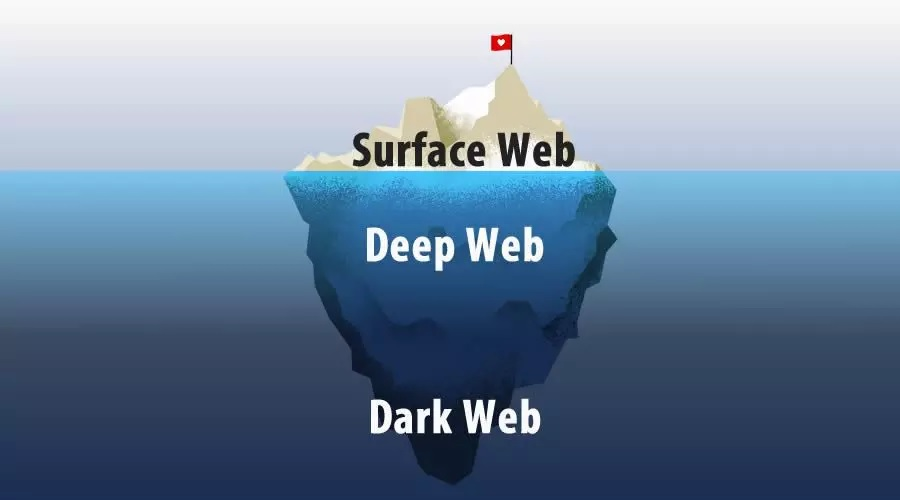
\includegraphics[width=0.8\textwidth]{Immagini/darkwebpic1.jpg}
	\caption{Livelli di Rete}
	\label{fig:onedarkweb}
\end{figure}

Come possiamo vedere il web di superficie è solo la punta visibile al di sopra del livello dell'acqua.
Sfortunatamente la maggior parte delle persone (aziende comprese) non competenti in ambito tecnologico o non a conoscenza di certi dettagli e informazioni, permettono l'indicizzazione dei propri dati. Ciò permette ad un'attaccante di raccogliere informazioni e ottenere l'accesso ai propri sistemi, a localizzare dati personali e molto altro.

\section{Struttura e Funzionamento}\label{sec:cap_sec_darkweb1}

Per poter accedere al dark web occorre utilizzare uno strumento in particolare: trattasi di Tor, The Onion Browser. Tor è stato progettato per assicurare una navigazione anonima sulle reti. Per accedere al dark web è necessario innanzitutto installare Tor Browser, utilizzabile esattamente come qualsiasi altro browser su sistemi quali Windows, Linux, macOS e device mobili. Il vantaggio di questo browser è la massima privacy garantita dalla navigazione in anonimato. 

Navigare nel dark web non è semplice per l’utente medio: occorre prestare la massima attenzione per evitare di incappare nei pericoli che contraddistinguono questo livello sommerso di Internet. Prima di poter accedere a qualsiasi contenuto presente nel dark web,è necessario conoscere gli indirizzi giusti: senza di essi non è possibile navigare nel web oscuro.

Una volta installato Tor è possibile accedere al dark web, utilizzando motori di ricerca quali Onionland o DuckDuckGo.

Il dark web viene considerato un grande sottoinsieme del deep web. Esso contiene decine di migliaia di indirizzi URL. Ogni pagina si distingue per il suo dominio .onion. Le pagine vengono ospitate da server che utilizzano i protocolli Tor. 

Si stima che il dark web rappresenti solo il 5\% della totalità di Internet. Questo universo nascosto risulta graficamente molto simile (seppur meno complesso ed esteticamente gradevole) al web superficiale e la navigazione è pressoché identica. La differenza sta nella struttura degli URL, che terminano con .onion piuttosto che con .com, .it o .eu. 

\begin{figure}[ht]
	\centering
	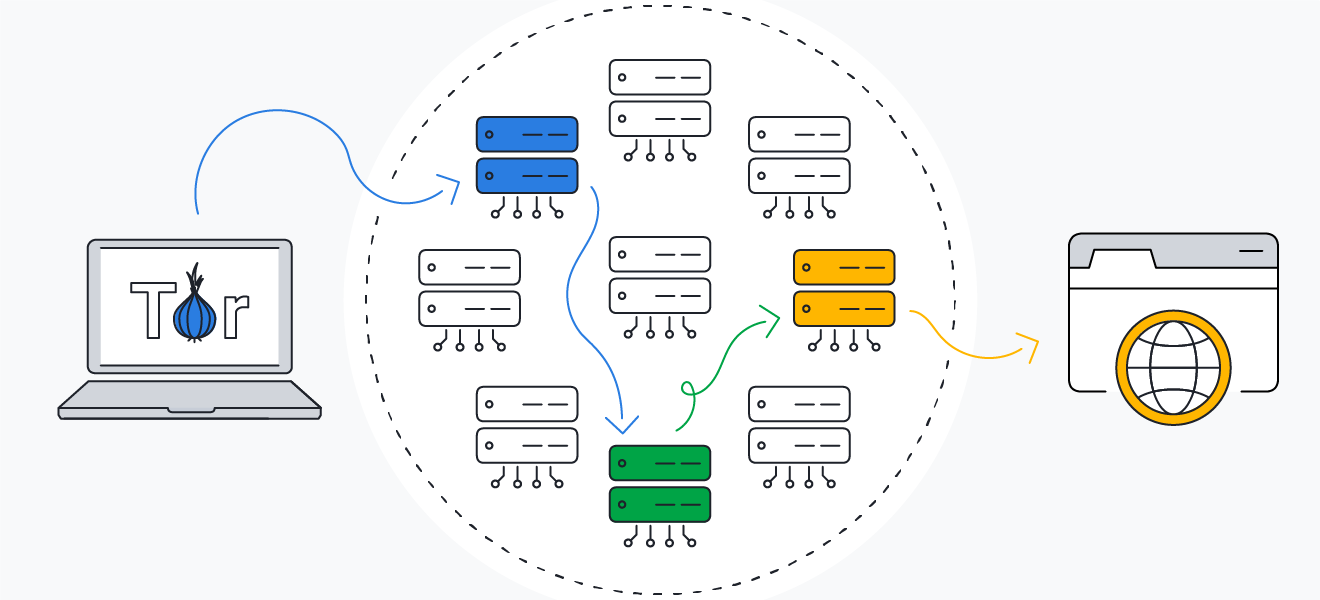
\includegraphics[width=0.8\textwidth]{Immagini/img-02.png}
	\caption{Instradamento di tor (tre nodi)}
	\label{fig:twodarkweb}
\end{figure}

Uno dei metodi più utilizzati per accedere e navigare nel deep web è Tor. Questo network decentralizzato è costituito da server, i cosiddetti relay, dislocati in ogni angolo del mondo. Questi relay, ovvero i nodi, vengono gestiti da utenti specializzati e volontari. Si stima che i nodi Tor siano tra i 6.000 e gli 8.000. Mentre sono circa 3.000 i ponti (bridge) offerti da Tor. 

I dati di navigazione, con Tor, non transitano dal client al server (come avviene durante una classica navigazione), ma i pacchetti di dati passano mediante i relay Tor che fungono da router. I relay realizzano un circuito virtuale crittografato a strati: una struttura a cipolla. Per questo, gli URL della rete Tor hanno un TLD (Top Level Domain) .onion, differente dal classico .com o .it.

Navigare sul deep web utilizzando Tor presuppone un processo particolare. Una volta aperto il browser Tor, sarà lo stesso browser a scegliere dall’elenco directory server la lista di nodi da utilizzare. La configurazione standard prevede tre nodi, scelti in modo casuale, i quali formano la catena di navigazione. Il circuito può essere consultato in tempo reale mediante la pagina del browser e può essere cambiato cliccando sul pulsante a sinistra della barra dell’URL. 

La comunicazione viene crittografata a qualsiasi livello della catena di navigazione. La crittografia si ripete lungo tutti i nodi: i nodi possono conoscere solo il nodo immediatamente precedente e immediatamente successivo, e nessuno degli altri. È quasi impossibile (o comunque molto complesso) risalire al client di partenza. È per questo che l’utente potrà navigare in anonimato. 

Il traffico Tor passa per almeno tre relay prima di raggiungere la destinazione: 

\begin{itemize}
\item Il guard relay, ovvero il nodo di guardia o di partenza;
\item Il middle relay, ovvero il nodo intermedio che riceve il traffico e lo passa al relay successivo;
\item L’exit relay, il nodo di uscita.
\end{itemize}


\'E poi fondamentale ricordare che il browser Tor non viene utilizzato solamente per navigare nel deep web e nel dark web (inaccessibile mediante i comuni motori di ricerca) ma anche per il surface web (in totale anonimato).

\section{Concetti di base del Dark Web}\label{sec:cap_sec_darkweb2}

Il dark web è quindi un contenitore di informazioni, basato sul web e caratterizzato da sistemi di comunicazioni anonimi, con lo scopo di proteggere utenti e la loro identità attraverso tecnologie, quali le comunicazioni criptate, la crittografia del traffico e il suo offuscamento.
Grazie alla sua massiccia garanzia dell'anonimato, il dark web è diventata pian piano il canale principale per lo scambio e la distribuzione di contenuti pericolosi, vietati o illegali.

Il Dark Web è diventato il principale strumento per veicolare questi contenuti grazie appunto alle sue caratteristiche. Troviamo tra i suoi principali usi quello dei marketplace illeciti (per l'acquisto di droghe, armi, materiale pornografico illegale, carte di credito rubate e documenti) e quello del Cybercrime-as-a-Service, in quanto è possibile interagire con fornitori di servizi illegali. Questa nuova industria di servizi per i cybercriminali ha modificato notevolmente il panorama delle minacce per le aziende di tutte le dimensioni. 

\newpage

In particolare attacchi ransomware \footnote{Programma informatico dannoso ("malevolo") che può “infettare” un dispositivo digitale, bloccando l’accesso a tutti o ad alcuni dei suoi contenuti, per poi chiedere un riscatto (“ransom”).}, phishing, cryptojacking e attacchi di tipo distributed denial-of-service (DDOS) per conto di altri, dietro pagamento di una commissione.

Il potere distruttivo e accattivante degli attacchi ransomware è dato dal fatto che nella maggior parte dei casi il fornitore del servizio prende semplicemente una percentuale dei profitti. Ciò significa che chiunque può sfruttare a pieno questi attacchi debilitanti senza bisogno di competenze IT o investimenti finanziari. 

I fornitori di Cybercrime-as-a-Service più sofisticati forniscono persino dashboard a cui i loro clienti possono accedere per monitorare il progresso e il tasso di successo della loro campagna di attacco.


\section{Differenze tra Deep Web e Dark Web}\label{sec:cap_sec_darkweb3}

Come detto in precedenza il web come lo conosciamo, comprende solo la parte indicizzabile e pubblicamente accessibile, consultabile tramite Google, Bing, Yahoo e altri motori di ricerca (Questo lato della rete contiene all'incirca 55 miliardi di pagine web).

Può sembrarci un numero davvero elevato, ma il numero di siti web presenti su internet non indicizzabili e non pubblicamente visibili è ancora più elevato, in questa parte della rete possono accedere solo governi, servizi militari e altre organizzazioni, ad esempio la NASA, questi servizi sono nascosti dal resto della società e l'insieme di questi contenuti forma il deep Web. Si stima che il deep web sia da 400 a 500 volte più grande del web di superficie.
Il dark web di cui abbiamo parlato finora, fa parte del cosiddetto deep web e fornisce anonimato e sicurezza a chiunque la visiti, il dark web, viene utilizzato per molteplici scopi, sia legali che illegali. Ed è costruita su una serie di reti sovrapposte. \footnote{Queste reti prendono il nome di Overlay Networks}

\begin{figure}[ht]
	\centering
	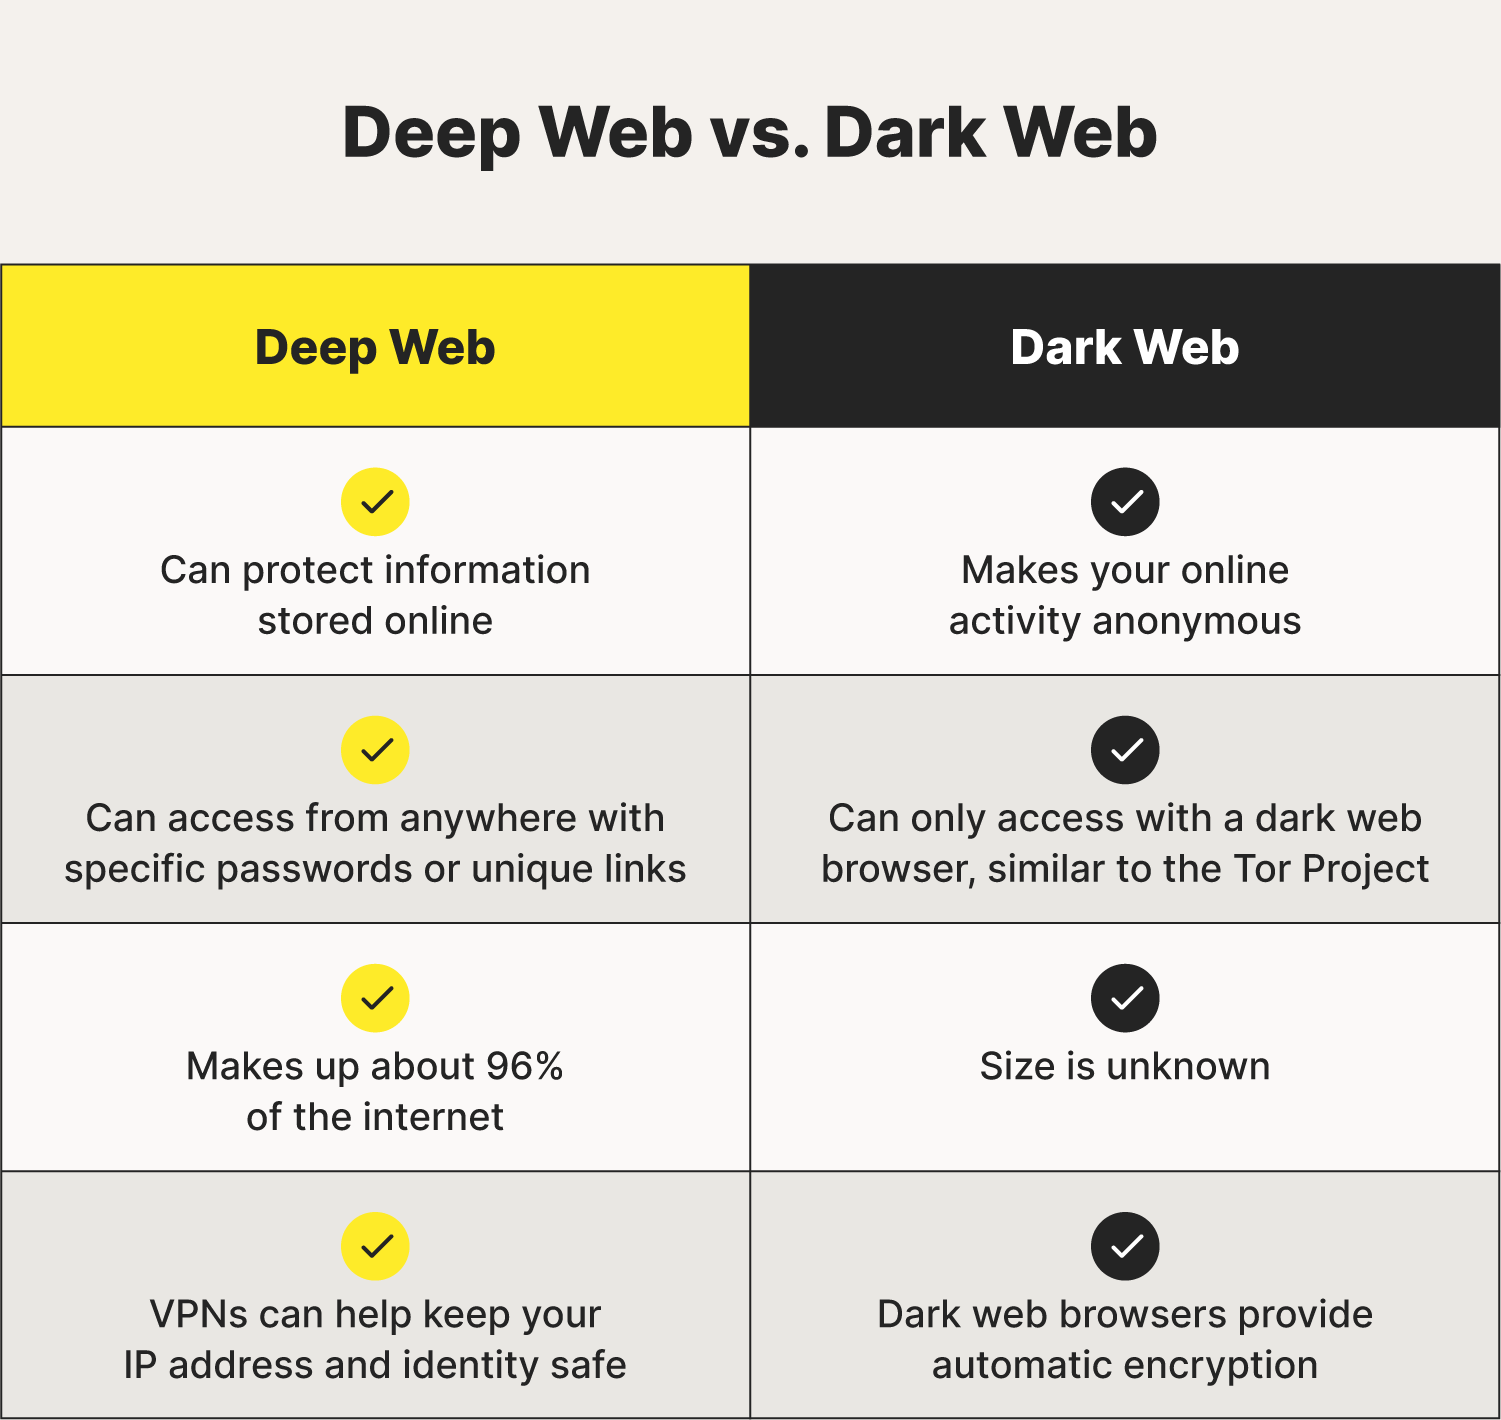
\includegraphics[width=0.8\textwidth]{Immagini/deep-vs-dark-web.png}
	\caption{Deep Web vs Dark Web}
	\label{fig:threedarkweb}
\end{figure}

\newpage
"So is there a difference between the invisible or deep web and Dark web?

Many people that know about the invisible web will give a different answer to this question because it is easy to consider them as being the same thing. Central to the Dark web discussion are key definitions to reduce the confusion concerning Deep web, Dark web and anonymous browsing. The Deep web is, in a sense, the content of databases and other services of the web that for one reason or another cannot be indexed by the typical search engines that everybody uses. The Deep web is not all bad. The Dark web on the other hand is part of the Deep web, and requires a specially designed browser and encryption methods to access. Neither the Deep nor Dark web can be indexed when seeking information which leads people to believe that they are the same. But the two categories of web that cannot be indexed are synonymous. The Dark web is a massive cyber underground world where some of the worst kinds of people like hackers, gangsters, terrorists, and pedophiles go to have fun or purchase anything. Some people might even consider the Dark web to be the black market where one can acquire things like drugs, counterfeit currency, forged documents, firearms and explosives, human organs, and even hitmen. One cannot expect to purchase these things by inputting a credit card number and providing an address to which to have it shipped. There are certain things that help Internet crime work. Forms of cryptocurrency, such as bitcoins, facilitate currency exchange for whatever the purchaser wishes. Many organized cybercrime syndicates even have the ability to outsource hackers for hire. There are sites on the invisible web where one can contract certain “entities” to hire a hacker to do the dirty work for a well-funded organization or person. As explained, one can see there is a difference, whether it is slight or not, between the Deep and Dark web. Both require special access but one is far more dangerous than the other. The Dark web (or Dark Net) is a twisted and maniacal place where some of the world’s most unsavory or dangerous people or groups centralize to stay “under the radar” of government agencies or others that may condemn their actions." \cite{darkweb3}

Possiamo quindi affermare che il dark web sia la parte più pericolosa e profonda del deep web, un enorme mondo "sotterraneo" dove diversi criminali, come hacker, gangster, terroristi e pedofili, vanno per divertirsi o acquistare qualsiasi cosa.
Il Dark web viene spesso considerato il mercato nero dove è possibile acquistare droghe, valuta contraffatta, documenti falsi, armi, esplosivi, organi e persino sicari. In questo ambiente vengono utilizzate criptovalute, come i bitcoin, per facilitare lo scambio.

Come spiegato, si può vedere come ci sia una differenza, sebbene minima o meno, tra deep web e dark web. Entrambi richiedono un accesso speciale, ma uno è molto più pericoloso dell'altro. Il dark web (o Dark Net) è un luogo perverso dove alcune delle persone o dei gruppi più pericolosi al mondo si centralizzano per rimanere "sotto il radar" delle forze dell'ordine.

La maggior parte dei contenuti del dark web può risultare estremamente inquietante, tuttavia esistono anche utilizzi rispettabili e legittimi di questa tecnologia.

Di seguito alcuni degli utilizzi legittimi:

\begin{itemize}
    \item SecureDrop è un software open-source per la comunicazione sicura di informazioni, utilizzato dalle organizzazioni mediatiche per ricevere documenti da fonti anonime in modo sicuro. Viene utilizzato tramite la rete Tor e nel tempo questo e altri servizi simili sono stati impiegati dall'Associated Press, The Washington Post, The New York Times, CBC, ProPublica e molte altre organizzazioni.
    \item Giornalisti che risiedono in stati con regimi repressivi usano Tor per comunicare con il mondo esterno e per poter diffondere ingiustizie sociali e le violazioni dei diritti umani che avvengono in determinati periodi di crisi o conflitto.
    \item Tor permette ad agenti delle forze dell'ordine di navigare e visitare siti e servizi sospetti senza lasciare tracce compromettenti. Questo perché nel caso in cui un indirizzo IP di un'agenzia governativa o delle forze dell'ordine fosse rilevato nei log del sito, rivelerebbe che il sito è sotto sorveglianza.
    \item Tor consente inoltre di eludere la censura statale. Un esempio significativo è rappresentato dal blocco dell'accesso a ProtonMail da parte della Turchia. \footnote{Nel mese di giugno 2020, imposto dal governo come parte delle restrizioni sulle comunicazioni, in linea con la politica di controllo delle comunicazioni digitali e della libertà di espressione} In quella circostanza, l'unico modo per i residenti turchi di accedere al servizio di posta elettronica sicuro e criptato era tramite il sito .onion di ProtonMail. \cite{darkweb4}
\end{itemize}

\section{Anonimato e Implicazioni di Sicurezza}\label{sec:cap_sec_darkweb4}

Ci sono diversi browser che vengono utilizzati per accedere al deep web, come già detto il più conosciuto è TOR browser. Tor (The Onion Router) è stato creato a metà degli anni 90 come risultato di un progetto condotto dall'US Naval Research Lab \footnote{Organizzazione di ricerca scientifica e ingegneristica della Marina degli Stati Uniti}, uno dei contributi più rilevanti del laboratorio è stato appunto lo sviluppo di Tor, una rete anonima progettata per proteggere la privacy degli utenti su Internet e con l'obbiettivo di garantire comunicazioni sicure per il governo statunitense, in particolare per i militari, le forze dell'ordine e i diplomatici che operano in aree in cui la privacy è cruciale.
Tor utilizza un sistema di "onion routing", dove il traffico dati viene crittografato in più strati e inoltrato attraverso una serie di nodi volontari in tutto il mondo, rendendo difficile il tracciamento dell'origine o della destinazione finale del traffico. Il progetto è diventato poi Open Source nel 2004.

Per garantire anonimato e sicurezza utilizza una serire di entry point randomici selezionati da una serie di server e le richieste vengono criptate e inoltrate insieme all'indirizzo di destinazione finale.
Ogni nodo successivo decripta l'indirizzo e cripta nuovamente la richiesta per poi inoltrarla (ogni nodo conosce solamente il nodo precedente e quello successivo). Al termine le informazioni raggiungono l'exit point da dove poi vengono indirizzate verso la loro destinazione finale.

\newpage

Inoltre, per garantire un livello di sicurezza maggiore i percorsi di instradamento vengono aggiornati approssimativamente ogni 10 minuti, per garantire maggior sicurezza nel caso in cui il traffico in corso sia monitorato.
Hornet è una rete di onion routing ad alta velocità che sfrutta un'archiettura di ultima generazione per rendere il tracking più complicato. \footnote{Hornet viene sviluppato da Chen Chen, del Carnegie Mellon University assieme a Daniele Enrico Asoni, David Barrera, George Danezis and Adrian Perrig}

Il funzionamento prevede l'attraversamento di diversi server creando passaggi virtuali, rendendo il tracciamento dell'IP un processo complesso. Ciò che rende Hornet più sicuro rispetto al browser TOR è che, quando Hornet è in uso, il sistema non memorizza gli stati delle sessioni, al contrario, Hornet trasferisce gli stati delle sessioni agli host finali per impostazione predefinita, criptando ogni pacchetto per ridurre il rischio di perdite di dati.

Recentemente è stato messo in discussione la protezione offerta dal browser TOR, in quanto nella realtà odierna esiste sempre almeno un individuo con competenze informatiche tali da poter violare qualsiasi rete su qualsiasi sistema, servendosi semplicemente di un dispositivo in grado di accedere alla rete e una connessione Internet.

"Una nuova ricerca del MIT (Massachusetts Institute of Technology) mostra come le entry guard "maligne" di TOR possano eliminare le funzionalità di anonimato del Dark Web, esponendo gli utenti e i siti web che visitano."

Il processo tramite la quale è possibile tracciare gli utenti di TOR è chiamato "website fingerprinting", quando un utente tenta di eseguire fingerprinting attack, deve iniziare con l'analizzare il comportamento di TOR  e della rete formatasi (quindi, i nodi che compongono il collegamento) quando avviene una connessione. Durante la fase di costruzione del circuito per la comunicazione tra un client e un servizio nascosto, TOR presenta schemi di traffico unici che permettono ad un avversario di identificare e correlare in modo efficiente e accurato i nodi coinvolti nella comunicazione.
Si andrà quindi a identificare i circuiti sospetti, per ridurre lo spazio di indagine ai soli servizi nascosti.

Un altro modo per tracciare un'utente è quello di monitorare i suoi keystroke, proprio come la grafia di ognuno è differente, anche quando si utilizza un computer è possibile differenziare un modello di keystroke dall'altro.

Il modo migliore per non essere tracciati è quello di avere un basso profilo e restare alla larga da attività illegali, in quanto nulla è davvero anonimo.

\newpage

Altri suggerimenti per rimanere il più anonimo possibile consistono nel:

Usare metodo di pagamento specifici, in particolar modo cryptovalute, quali Bitcoin (BTC) e Monero, questo perché sono le monete più facili da ottenere e scambiare, e perché Monero può essere acquisto solo utilizzando un'altra criptovaluta. 

L'utilizzo di una Virtual Private Network (VPN) prima di accedere al browser. Questo andrà a mascherare l'indirizzo IP dell'utente aggiungendo un ulteriore livello di sicurezza e anonimato.

Sarà poi necessario individuare gli URL .onion di interesse, tramite specifiche directory e forum sul dark web, lasciando il minor numero di tracce possibili.

\'E fondamentale non scaricare file sconosciuti o fare clic su annunci, in quanto queste semplici azioni potrebbero dare il via ad una serie di attacchi informatici, con download falsi e potenzialmente infettati da diversi malware e virus.

\begin{figure}[ht]
	\centering
	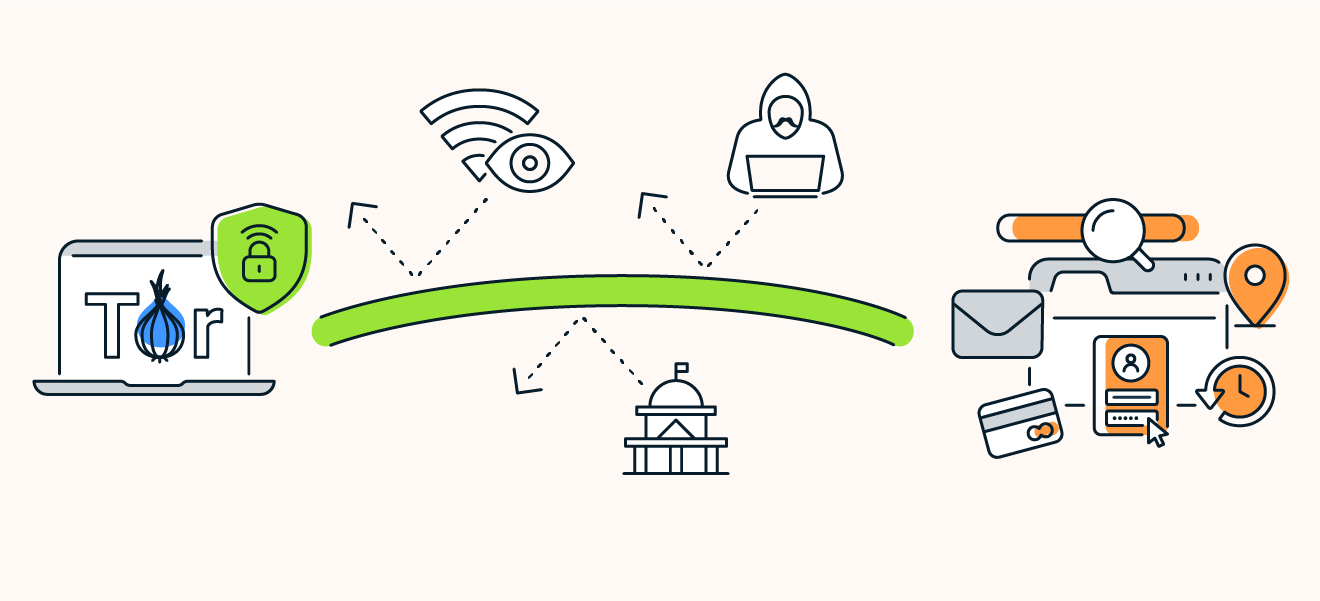
\includegraphics[width=0.8\textwidth]{Immagini/Academy-Tor-browser-03.png}
	\caption{Utilizzo di Tor e le VPN per il traffico criptato}
	\label{fig:fourdarkweb}
\end{figure}

\'E fortemente consigliato il collegamento ai soli siti HTTPS. In cui i dati vengono trasmessi in forma crittografata, tramite l'utilizzo di un certificato SSL. TOR non utilizza lo stesso certificato ma questa precauzione è da considerare sul web di superficie.

\'E fondamentale non rivelare mai informazioni personali quali nome, indirizzo, numero di telefono, email e profili sui social media.

In fine l'utilizzo di software Antivirus.
